\chapter{Mise en place du protocole de communication}
	Le premier chapitre de se rapport a présenté les principales idées que l'on souhaite mettre en 
	place pour avoir une architecture d'objets dynamique et générique. On va maintenant s'intéresser
	à la manière dont on peut les réaliser.


\section{Les protocoles existants}
	Il existe une multitude
	% A ECRIRE, A ECRIRE	, A ECRIRE, A ECRIRE, A ECRIRE, A ECRIRE

	\subsection{Zigbee}
	% A ECRIRE, A ECRIRE	, A ECRIRE, A ECRIRE, A ECRIRE, A ECRIRE
	\subsection{Z-Wave}
	% A ECRIRE, A ECRIRE	, A ECRIRE, A ECRIRE, A ECRIRE, A ECRIRE
	\subsection{Alljoyn}
	% A ECRIRE, A ECRIRE	, A ECRIRE, A ECRIRE, A ECRIRE, A ECRIRE
	
	% IMPORTANT : explication de pourquoi on a pas pris un protocole existant :
	%  - ne correspond pas forcément à toute les fonctionnalités que l'on souhaite mettre en place
	%  - est difficilement adaptable avec les outils que l'on a (mbed, attiny, bluetooth Bolutek)

\section{Le réseau virtuelle}
	Nous allons maintenant nous intéresser aux caractéristiques du protocole qui a été
	développé dans ce projet. L'un des points clés de la mise en place d'objets pour la domotique 
	est la communication avec ceux-ci. Ces objets doivent en effet être "connectés" pour que l'on
	puisse les contrôler ou recevoir des messages de leur part. Il est donc nécessaire de mettre en 
	place une architecture réseau qui puisse lier ces objets de façon efficace. Mais la mise en place
	de ce réseau n'est pas forcément évidente. Si l'on souhaite être indépendant du support de 
	communication, il faut mettre en place des moyens de lier des objets de supports différents. Il 
	est également possible de communiquer avec des objets mobiles. Cela signifie que l'architecture 
	du réseau doit également être dynamique. C'est pourquoi il est indispensable d'avoir un protocole
	capable de gérer ces détails.
	
	\subsection{Architecture du réseau}
% 		définition d’un réseau (uniquement 1 support de communication)
% 		description de la connexion des réseaux
% 		exemples d’architecture de réseau virtuel
		Pour bien comprendre comment est structuré un réseau d'objets, il faut d'abord s'intéresser 
		à une architecture simple ne faisant qu'intervenir un seul support de communication.
		
		\begin{figure}[!ht]
         \centering
         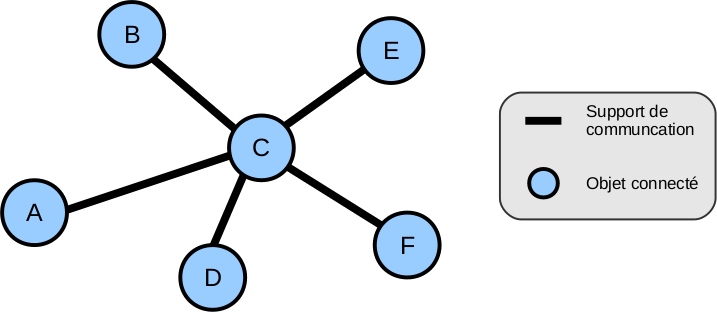
\includegraphics[width=.8\textwidth]{img/reseau_etoile.png}
         \caption{Exemple d'architecture réseau d'un point d'accès Wifi (architecture en étoile).}
         \label{testEffibox}
      \end{figure}

	\subsection{Le routage}
% 		présentation du protocole VIP
% 		explication du transfert d’un message d’un support à un autre
% 		exemple concret d’un envoi de message
	\subsection{Un réseau dynamique}
% 		apparition, disparition ou déplacement d’objets dans le réseau
% 		présentation du protocole VARP
% 		exemple d’apparition d’un objet
% 		les objets mobiles

\section{La généricité des objets connectés}
% 	explication de l’intérêt de classifier les actions
	\subsection{Méthode de classification des actions sur les objets}
% 		recherche des informations caractérisant les actions
% 		algorithmes de classification
	\subsection{La structure actuelle}
% 		explication du choix de la hiérarchie actuelle d’actions
% 		les limites et les défauts de cette hiérarchie
	\subsection{Gestion dynamique d’objets inconnus}
% 		comment un objet d’un nouveau type peut s’intégrer à la hiérarchie
% 		les différentes solutions d’intégration
% 		exemple

